\documentclass[11pt]{article}
\usepackage[T1]{fontenc}
\usepackage[utf8]{inputenc}
\usepackage{lmodern,amsmath,amssymb,booktabs,array,graphicx}
\usepackage[margin=1in]{geometry}
\usepackage{microtype}
\usepackage{pgfplots}
\usetikzlibrary{arrows.meta}
\pgfplotsset{compat=1.18}
\usepackage[colorlinks=true,linkcolor=blue!50!black,citecolor=blue!50!black,urlcolor=blue!50!black]{hyperref}
\usepackage{placeins}
\setlength{\parskip}{4pt}
\setlength{\parindent}{0pt}
\newcommand{\D}{\mathrm{D}}
\newcommand{\R}{\mathrm{R}}
\title{Inherited Action Preferences in a Resource-Limited Artificial Ecology:\\Controls, Relearning, and Update Allocation}
\author{Xuening Wu\\Pfizer, Shanghai, China\\\small\href{mailto:xuening.wu@pfizer.com}{\texttt{xuening.wu@pfizer.com}}}
\date{30 September 2026}
\begin{document}
\maketitle
\begin{abstract}
Passing learned parameters to offspring can accelerate adaptation, but random controls may confound update direction with the structure, magnitude, and timing of hereditary change. We examine these distinctions in a resource-limited spatial artificial ecology with lifetime action-value learning and local reproduction. A state-preserving randomization retains each state's update mean and action-contrast norm. With 512 fixed-norm updates, directed inheritance establishes in 20 of 20 runs versus 18 of 20 under this control, with a paired capped-time advantage of 4,870 sweeps; weaker whole-table controls establish in only two and zero runs. Erasing newborn action preferences reduces directed attainment to six of 20, while faster newborn learning restores 20 of 20, supporting a relearning-related mechanism in that regime. Continuous proportional writeback retains a speed advantage under common step-size and parameter-range constraints. However, a population-wide update quota ends writeback at different times in the two evolving populations. At one energy allocation, replacing a 1,024-event cutoff with a common time cutoff changes the ranking, while also changing realized update amounts. A separate fixed-step experiment matches all 1,024 updates and their cumulative magnitudes: staged release improves directed mean occupancy by 8.25 percentage points, but no group reaches the prespecified establishment threshold. These findings support conditional benefits of inherited action preferences and expose the roles of control geometry, newborn expression, and update allocation. They do not establish a universal inheritance advantage, a pure timing mechanism, or increased long-term evolvability.
\end{abstract}

\section{Introduction}
Learning and inheritance operate on different timescales. An individual can adjust its behavior during its lifetime, whereas reproduction initializes offspring that must act under their own local conditions. Directly retaining a parent's learned parameters offers an apparent shortcut, but its performance depends on what is retained, how offspring continue learning, and how behavior affects survival and reproduction. Demonstrating a benefit in one setting leaves its mechanism and range of applicability unresolved.

These questions have a substantial history. Learning can guide evolution without direct transmission of acquired traits, as demonstrated in work on the Baldwin effect \cite{hinton1987}. Formal models also compare environmentally induced variation, random variation, and feedback from phenotype to inherited state \cite{rivoire2014}. In evolutionary robotics, inherited controllers have been compared with learning from scratch under different learning budgets \cite{jelisavcic2019}; subsequent work examines newborn performance and body--controller matching \cite{luo2023}. We therefore do not treat either direct writeback or reduced relearning as a new general principle.

The present study asks a narrower experimental question: what remains of a directed inheritance benefit after the random control preserves the state structure of the learned change, and how does that benefit depend on newborn expression and continued hereditary updating? A random perturbation can have the same total Euclidean norm as a learned update while allocating its components to different states. If some represented states cannot be encountered, equal global norm need not mean comparable opportunity to influence behavior. Conversely, preserving the state support still does not make trajectories or accumulated learning identical after populations diverge.

We investigate these distinctions in a deliberately simple artificial ecology. Individuals occupy a two-dimensional torus, choose among resting, harvesting, and dividing, and learn immediate local action values. Resource replenishment, action costs, stochastic mortality, and local reproduction determine population occupancy without an externally imposed population-level fitness selection operator. A hereditary table $g$ is separated from the lifetime table $\theta$. Reproduction can transmit part of $\theta-g$ to the child. The model is a computational testbed, not a calibrated account of biological cells.

Three initial experimental components provide complementary evidence. First, fixed-norm updates compare inherited direction with a state-preserving random alternative across update quotas. Second, a branch intervention removes newborn action preferences once the hereditary update quota is reached and tests whether faster lifetime learning compensates for their removal. Third, the original proportional update is evaluated with continuous writeback and with a finite update quota. The first component constrains variation magnitude; the second intervenes on expression; the third checks whether an observed benefit survives removal of the fixed-norm intervention. These components estimate distinct effects (Figure~\ref{fig:overview}). Follow-up experiments impose symmetric stability constraints and compare event quotas with common time cutoffs and fixed-budget release schedules.

Our contribution is the resulting control and intervention analysis. Stronger random controls substantially reduce the observed gap in establishment frequency while retaining a speed advantage in several fixed-norm settings. Newborn preference erasure and learning-rate compensation support a relearning-related mechanism in the tested fixed-norm regime. Finally, continuous and quota-limited writeback can yield opposite rankings at the same energy allocation, but follow-up interventions show that this comparison depends on the allocation rule and its coupling to reproduction. A matched-budget timing experiment supports an occupancy effect without confirming its primary establishment prediction. This evidence bounds a model-specific benefit rather than demonstrating a new hereditary channel, an evolutionary phase transition, or a general increase in evolvability.


\begin{figure}[htbp]
\centering
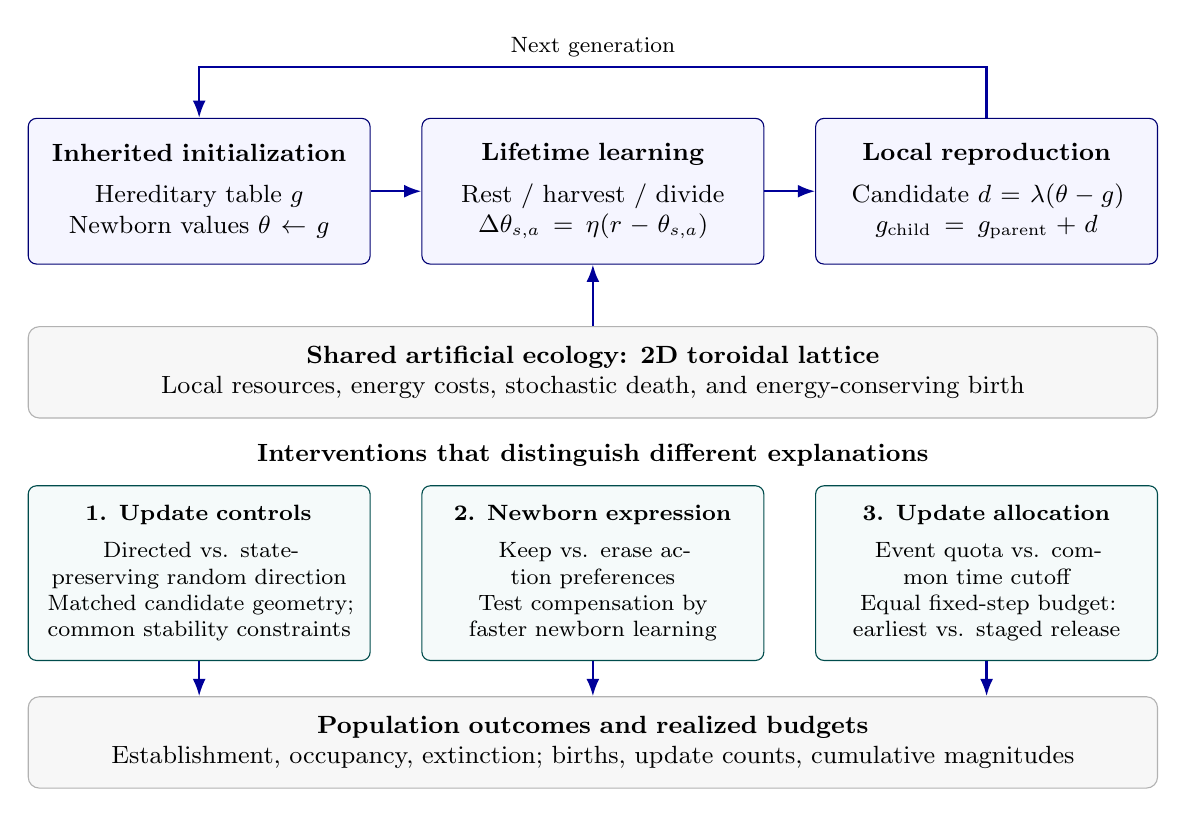
\begin{tikzpicture}[
  box/.style={draw=blue!45!black,rounded corners=3pt,fill=blue!4,
    text width=3.85cm,minimum height=1.85cm,align=center,inner sep=7pt,font=\small},
  test/.style={box,draw=teal!60!black,fill=teal!4,minimum height=2.05cm,font=\footnotesize},
  flow/.style={-{Latex[length=2.2mm]},thick,draw=blue!60!black}]
\node[box] (birth) at (0,0) {\textbf{Inherited initialization}\\[4pt]
Hereditary table $g$\\Newborn values $\theta\leftarrow g$};
\node[box] (learn) at (5,0) {\textbf{Lifetime learning}\\[4pt]
Rest / harvest / divide\\$\Delta\theta_{s,a}=\eta(r-\theta_{s,a})$};
\node[box] (child) at (10,0) {\textbf{Local reproduction}\\[4pt]
Candidate $d=\lambda(\theta-g)$\\$g_{\rm child}=g_{\rm parent}+d$};
\draw[flow] (birth.east)--(learn.west);
\draw[flow] (learn.east)--(child.west);
\draw[flow] (child.north)--++(0,.65)-|node[pos=.25,above,font=\footnotesize]{Next generation} (birth.north);
\node[draw=gray!60,rounded corners,fill=gray!6,text width=13.85cm,minimum height=1.05cm,
 align=center,font=\small,inner sep=7pt] (eco) at (5,-2.3)
 {\textbf{Shared artificial ecology: 2D toroidal lattice}\\
 Local resources, energy costs, stochastic death, and energy-conserving birth};
\draw[flow] (eco.north)--(learn.south);
\node[font=\small\bfseries] at (5,-3.35) {Interventions that distinguish different explanations};
\node[test] (geometry) at (0,-4.85)
 {\textbf{1. Update controls}\\[4pt]
Directed vs. state-preserving random direction\\
Matched candidate geometry; common stability constraints};
\node[test] (expression) at (5,-4.85)
 {\textbf{2. Newborn expression}\\[4pt]
Keep vs. erase action preferences\\
Test compensation by faster newborn learning};
\node[test] (allocation) at (10,-4.85)
 {\textbf{3. Update allocation}\\[4pt]
Event quota vs. common time cutoff\\
Equal fixed-step budget: earliest vs. staged release};
\node[draw=gray!60,rounded corners,fill=gray!6,text width=13.85cm,
 minimum height=1.05cm,align=center,font=\small,inner sep=7pt] (measure) at (5,-7)
 {\textbf{Population outcomes and realized budgets}\\
Establishment, occupancy, extinction; births, update counts, cumulative magnitudes};
\draw[flow] (geometry.south)--(geometry.south |- measure.north);
\draw[flow] (expression.south)--(measure.north);
\draw[flow] (allocation.south)--(allocation.south |- measure.north);
\end{tikzpicture}
\caption{Study overview. Individuals learn local action values during life and can transmit acquired changes at reproduction. The upper row shows the unmodified proportional rule with $\mu=0$, as in the central experiments. Fixed-norm, random-direction, and bounded variants intervene on the transmitted increment. The three intervention families test control structure, newborn expression, and update allocation; they estimate distinct effects. Stopping new writeback leaves lifetime learning and inheritance of existing $g$ active. The schematic shows the experimental design, not a universal benefit or a proven mediation pathway.}
\label{fig:overview}
\end{figure}

\section{Related work}
\paragraph{Learning and inheritance.}
The Baldwin effect concerns learning-mediated evolutionary change without directly encoding the acquired adjustment in offspring; direct writeback is a Lamarckian computational mechanism. Hinton and Nowlan provide a classic example of the former \cite{hinton1987}. Rivoire and Leibler explicitly compare ways of generating and transmitting variation, including phenotype-to-genotype feedback and environmental information \cite{rivoire2014}. Our use of separate inherited and lifetime tables instantiates a chosen architecture; it does not establish that architecture's biological existence or novelty.

\paragraph{Inherited learning in robots.}
Jelisavcic et al. compare inherited controllers with learning from scratch under different evaluation budgets \cite{jelisavcic2019}. Luo et al. investigate inherited learned traits, including newborn performance and a random-body comparison \cite{luo2023}. More recently, de Bruin et al. investigate parental sample reuse within Bayesian optimization under a low controller-learning budget \cite{debruinSamples}. These studies preclude interpreting reduced repeated learning as a new general finding. Our comparison instead preserves a candidate update's state-wise geometry, and our newborn intervention changes expressed action preferences while keeping inherited parameters fixed after the quota. The hereditary event quota here is also distinct from a controller's evaluation budget.

\paragraph{Learning and search allocation.}
Lamarckian and Baldwinian evolutionary algorithms can differ even on fixed objective functions. A recent empirical and runtime analysis identifies settings in which Baldwinian evolution outperforms Lamarckian evolution \cite{benito2026}. Thus an inheritance disadvantage in an externally stationary setting is not itself novel. Our event-allocation intervention differs from removing local learning: lifetime updates continue after new hereditary writes stop.

\paragraph{Ecology and benefit boundaries.}
Learning, resource competition, and reproduction already coexist in spatial agent models \cite{aguilar2019}. Thomsen and Rasmussen compare Darwinian, Baldwinian, and Lamarckian agents that acquire resources before reproducing, with outcomes affected by learning and replication costs \cite{thomsen2023}. Their fixed-size, nonspatial population differs from our variable occupancy and local resource depletion, but resource-dependent rankings are not new in themselves. Recent robot studies examine environmental conflict and predictability \cite{debruinDynamic}, and reduced inheritance benefits under pressure for morphological novelty \cite{muff2026}. Our external ecological rules remain fixed within a run; the boundary intervention is whether hereditary updating continues. We make no claim that these distinct experiments establish a common universal law. The novelty assessment is a targeted comparison with these works, not proof of the absence of other related designs.

\section{Model and experimental methods}
\subsection{Spatial ecology}
The lattice has $L=32$ sites per side and periodic boundaries. Each site contains at most one individual and a resource value $R_i\in[0,1]$. Initially, sites are independently occupied with probability $0.25$, occupied individuals have energy $E=1.5$, and all sites start with a resource value of one. Each sweep begins by replenishing every site's resource by $0.06$, capped at one, and then selects $L^2$ sites with replacement. Selecting an empty site does nothing. At an occupied site, background mortality occurs with probability $0.002$ before an action is chosen. Mortality is stochastic, with no fixed age limit; an individual may be selected multiple times or not at all in a sweep.

The available actions are rest, harvest, and divide, with respective energy costs $0.04$, $0.08$, and $0.12$. Harvest removes $\min(0.5,R_i)$ units of local resource and adds the same amount to the individual's energy, which is capped at four. A divide action succeeds if energy after its action cost exceeds two and at least one of the eight Moore neighbors is empty. An empty neighbor is selected uniformly. A fraction $f$ of the post-cost energy goes to the child and $1-f$ remains with the parent, conserving their total. Baseline $f=0.5$ is compared with $0.35$ or $0.65$ in specified experiments. Nonpositive post-action energy causes death. Individuals do not move.

\subsection{State, action selection, and lifetime learning}
Each individual carries an inherited table $g$ and a lifetime table $\theta$. Energy and resource are uniformly binned into eight bins each, and a binary variable records whether division would currently be feasible. The resulting $8\times8\times2=128$ states have three action values each. A sensitivity analysis uses $4\times4\times2$ states, with the same ecological engine. Both tables are initially zero in founders, and normally $\theta_{\rm child}=g_{\rm child}$ at birth.

With probability $0.05$ an individual chooses uniformly among the three actions; otherwise it chooses uniformly among actions with maximal values in the current row of $\theta$, treating values within $10^{-12}$ as ties. The selected coordinate is updated by
\begin{equation}
\theta(s,a)\leftarrow\theta(s,a)+\eta\{r-\theta(s,a)\},\qquad \eta=0.2.
\end{equation}
This is immediate action-value learning without a next-state bootstrap, not discounted-return Q-learning. Let $E_{\rm retained}$ be surviving post-action energy, including parent and child energy when division occurs, and zero after energy death. The reward is
\begin{equation}
r=E_{\rm retained}-E_{\rm before}+b\,\mathbf1_{\rm birth}-0.5\,\mathbf1_{\rm energy\ death},
\end{equation}
where the baseline birth bonus is $b=0.2$. Background deaths receive no action update. The learning update occurs before a successful birth copies the parent's learned table. Local reward is not population fitness, and a successful division can be locally reinforced even when repeated division has unfavorable ecological consequences.

\subsection{Hereditary update and random controls}
The original, or \emph{native}, writeback is
\begin{equation}\label{eq:native}
d=\lambda(\theta_{\rm parent}-g_{\rm parent}),\qquad
g_{\rm child}=g_{\rm parent}+d+\epsilon_{\mu}.
\end{equation}
Here $\epsilon_{\mu}$ denotes an independent mutation increment. All central experiments reported here set $\mu=0$, so $\epsilon_{\mu}=0$; they do not estimate a mutation--writeback phase diagram. Native writeback uses $\lambda\in\{0.25,0.5,1\}$. A no-writeback reference sets $\lambda=0$ while retaining lifetime learning. This reference is not an independent-mutation evolutionary algorithm.

For a nonzero candidate in the fixed-norm experiment, the transmitted step is rescaled to
\begin{equation}\label{eq:fixed}
d_q=q\frac{\theta-g}{\|\theta-g\|_2},\qquad q=0.1841261006694567.
\end{equation}
The value of $q$ was carried forward from the earlier study stage and held fixed across the reported confirmation, representation, and robustness conditions. It was not retuned for the coarser representation. In the fixed-norm implementation, candidate norms below $10^{-12}$ are treated as zero and skipped without consuming quota; no such skips occurred in the reported formal main conditions. Native updates have no corresponding minimum-norm floor. Equation~\ref{eq:fixed} is a direction intervention, not a reparameterization of a single fixed $\lambda$.

For any state's three candidate components $d_s$, decompose
\begin{equation}
m_s=\tfrac13\mathbf1^\top d_s,\qquad c_s=d_s-m_s\mathbf1.
\end{equation}
Our main random control samples $\phi_s$ uniformly from $[0,2\pi)$ in the two-dimensional zero-sum plane and constructs
\begin{equation}\label{eq:rotation}
\widetilde d_s=m_s\mathbf1+\|c_s\|_2(\cos\phi_s\,u+\sin\phi_s\,v),\quad
u=\frac{(1,-1,0)}{\sqrt2},\quad v=\frac{(1,1,-2)}{\sqrt6}.
\end{equation}
The operation preserves each row's mean, contrast norm, and full norm, and does not turn an all-zero row into a nonzero row. It randomizes action preference within states, not the states receiving updates. It does not preserve the sparsity of individual actions within a row.

This control retains state-level learning information. The matching is with the candidate from the same parent in that run; two evolving populations need not have equal state visitation, identical parents, or equal cumulative row-wise changes. We therefore use ``state-preserving randomization'' rather than an information-free mutation control. Whole-table shuffled and isotropic controls, each with the same total fixed norm, provide diagnostic comparisons. The shuffled control permutes candidate coordinates and applies independent random signs; the isotropic control normalizes an independent Gaussian vector. Near-zero candidates trigger an isotropic step in these weaker controls, rather than a skip; no near-zero candidate skips were recorded in the formal directed or state-preserving conditions. Their movement of updates across states is part of what the stronger control removes.

A quota $B$ limits the number of nonzero hereditary updates across the population, not births or learning interactions. After quota exhaustion, reproduction and lifetime learning continue, but offspring receive unchanged parental $g$. If a run uses all $B$ fixed-norm updates, its sum of update norms and sum of squared update norms are $Bq$ and $Bq^2$. These are not the net genome displacement and are not Shannon information. Early extinction can prevent quota exhaustion. Under native writeback even equal update counts do not equalize these magnitude totals.

\subsection{Newborn expression intervention}
The mechanism experiment uses fixed-norm updates and $B=512$. For each direction and seed, branches have identical histories until the quota is consumed. Starting with the birth that consumes the 512th update, all subsequent newborns either retain $\theta=g$ or have their expressed values replaced by the per-state mean,
\begin{equation}
\theta_{\rm child}(s,a)=\tfrac13\sum_{a'}g_{\rm child}(s,a').
\end{equation}
The latter erases newborn action preferences while preserving each state's mean value and the hereditary table itself. No further hereditary updates occur, and already-existing individuals are unchanged. For these newborns only, the learning rate is set to $\eta_c\in\{0,0.2,0.8\}$. This changes update weight without adding interactions or energy.

The main intervention contrast is erase minus keep at $\eta_c=0.2$ within each hereditary direction. Compensation is assessed by how the erase--keep loss changes at $\eta_c=0.8$. The zero-learning condition is an auxiliary limit. The two directions reach their quotas in different ecological states, so within-direction branch interventions do not constitute a complete mediation decomposition of the between-direction effect.

\subsection{Symmetric constraints and allocation diagnostics}
For the stability follow-up, both same-parent candidate updates receive a common global multiplier that caps their full norm at $Q=0.1841261006694567$. For bounded variants, each state's pair receives a further common multiplier that keeps both candidate offspring within the same coordinate range; a 1\% interior slack is used when a boundary constrains the step. We compare the original rule, the norm cap alone, the range $[-0.62,0.42]$, and the wider range $[-1,1]$. The narrower range follows the baseline reward bounds and zero initialization. These transformations preserve same-parent row matching but modify proportional writeback; they do not match the histories of different populations or their behavioral changes.

At $f=0.65$, $\lambda=1$, the common-time diagnostic retains the narrower range and compares continuous writing, a 1,024-event quota, and common cutoffs after 150 or 750 complete sweeps. The times were fixed from earlier cutoff audits before the new seed block. Learning and inheritance of existing $g$ continue after new writes cease. The primary contrast is the change in the directed capped-time advantage under the 750-sweep rule relative to the event quota.

A separate allocation experiment normalizes each nonzero learning difference to $q=0.02$ before constructing its paired random candidate. This conservative step was fixed from the preceding update-size audit, not tuned on the new seeds. An opportunity is skipped without debiting the quota if either same-parent candidate cannot retain this norm inside the common narrower range. Random directions are drawn once per birth, not resampled until feasible. One schedule makes all 1,024 events available initially; the other releases 128 at internal times $0,107,214,321,429,536,643,750$, with unused credits carried forward until the run ends. The last tranche is available from sweep 751. The primary prediction is faster directed establishment under staged release; occupancy AUC is secondary. This is a fixed-step intervention, not a replication of natural proportional magnitudes.

\subsection{Design, endpoints, and statistical unit}
All formal runs last 20,000 sweeps, with occupancy sampled every 200 sweeps including time zero. The primary endpoint is the first sampled time $t_j$ for which all five samples $t_j,\ldots,t_{j+4}$ have occupancy at least $0.95$. The five samples span 800 sweeps. Occupancy between samples is unobserved, and attainment does not guarantee that occupancy remains above the threshold thereafter. If no such span occurs, the endpoint remains unreached and the reported capped time $T^*$ is 20,000. This value is not an estimate of the unobserved time to eventual establishment.

We also report attainment counts, extinction, the trapezoidal area under the occupancy curve (AUC) divided by 20,000, and mean occupancy at the final five samples strictly after sweep 19,000. Thresholds 0.90 and 0.99 are auxiliary sensitivity endpoints. Runs are never removed for extinction, failure to establish, or incomplete quotas. Simulated descendants and repeated time points are not independent replicates.

The formal seed blocks are disjoint between study stages. Within a stage, the same seeds are paired across conditions, but shared seeds do not imply identical post-divergence ecological events. Comparisons use 20 seed pairs and 20,000 paired bootstrap resamples to obtain descriptive 95\% percentile intervals. Unless otherwise stated, bracketed ranges in the results denote these intervals. These intervals are not adjusted for multiple comparisons; we do not use them to claim family-wise significance, equivalence, or universal superiority.

\begin{table}[htbp]\centering\small
\caption{Formal experiment inventory. Counts are condition runs, not independent seeds. Shared no-writeback references are counted once per specified setting.}
\begin{tabular}{p{3.7cm}p{6.2cm}r}\toprule
Stage / seed block & Conditions & Runs\\\midrule
Control confirmation / 51000--51019 & Four update methods without quota, plus no writeback &100\\
Quota comparison / 52000--52019 & Four methods at five quotas; shared no writeback &420\\
Representation / 61000--61019 & Two binnings, two quotas, two directions; references &200\\
Expression / 62000--62019 & Two directions, two expressions, three newborn learning rates &240\\
Ecological sensitivity / 63000--63019 & Six settings, two directions and no writeback &360\\
Native connection / 81000--81019 & Two energy shares, two quota rules, three strengths, two directions; references &520\\
Symmetric stability / 101000--101019 & Four rules, six parameter settings, two directions; bounded quota follow-up &1200\\
Common cutoff / 102000--102019 & Four allocation rules, two directions &160\\
Fixed-budget release / 104000--104019 & Two release schedules, two directions &80\\\bottomrule
\end{tabular}\label{tab:inventory}
\end{table}

The synthesis contains 3,280 formal condition runs across nine blocks, including 1,440 runs in the three follow-ups. Development batches (45, 80, and 52 runs for the three archived experiment packages) and replay checks are excluded. The sequence was motivated by earlier exploratory results; it is not one prospectively registered study. Each later package records its local execution protocol and source hashes before its formal batch. The fixed-norm expression experiment, in particular, should not be represented as a mechanism confirmation performed under the native rule.

\section{Results}
\subsection{Control geometry changes the apparent benefit}
In the fixed-norm confirmation without an update quota, directed inheritance and state-preserving randomization both establish in 20/20 runs. Their mean establishment times are 1,290 and 3,040 sweeps, respectively. The paired mean random-minus-directed difference is 1,750 [1,650, 1,850] sweeps. Because update counts differ in this continuous experiment, this is not a comparison at equal cumulative variation.

At $B=512$, both main directions use their entire fixed-norm quotas. Directed inheritance establishes in 20/20 runs and the state-preserving random control in 18/20, with mean capped times 2,290 and 7,160. The paired difference is 4,870 [3,040, 7,120] sweeps. Both methods have zero extinctions. In the same seed block, whole-table shuffling establishes in 2/20 runs and isotropic variation in 0/20 (Figure~\ref{fig:control}). Thus the magnitude of the apparent benefit depends strongly on the chosen random control. The 20/20 versus 18/20 outcome alone is not sufficient to assert a population-level difference in establishment probability.

The weak random controls allocate approximately one quarter of their squared update mass to physically unreachable represented states, whereas the main state-preserving control allocates none. This audit demonstrates a structural mismatch, but does not isolate unreachable mass as the sole reason for weaker performance: global shuffling and isotropic variation also change other aspects of the state--action structure.

\begin{figure}[htbp]\centering
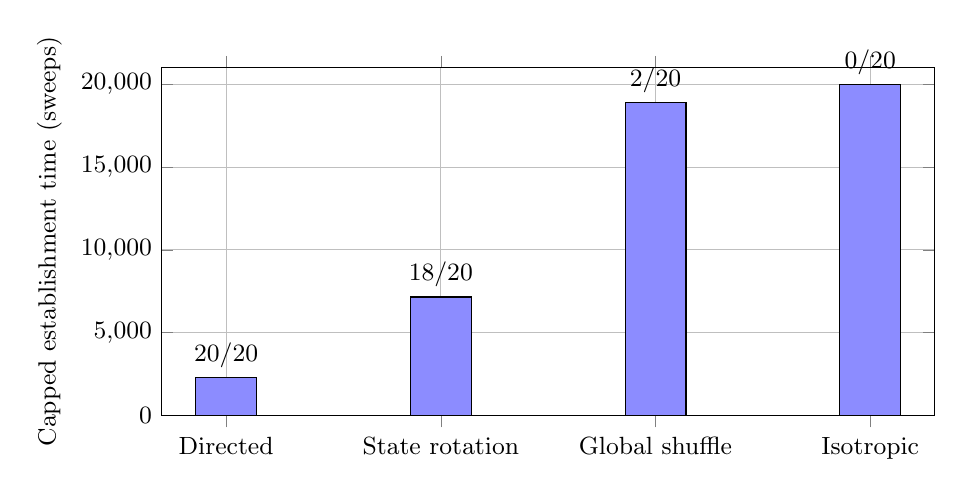
\begin{tikzpicture}\begin{axis}[width=0.94\linewidth,height=6cm,ymin=0,ymax=21000,scaled y ticks=false,ytick={0,5000,10000,15000,20000},ylabel={Capped establishment time (sweeps)},grid=major,legend style={at={(0.5,1.03)},anchor=south,legend columns=2,font=\small},tick label style={font=\small},label style={font=\small},ybar,bar width=22pt,xtick={1,2,3,4},xticklabels={Directed,State rotation,Global shuffle,Isotropic},nodes near coords,point meta=explicit symbolic,every node near coord/.append style={font=\small}]\addplot[fill=blue!45] coordinates {(1,2290) [20/20] (2,7160) [18/20] (3,18910) [2/20] (4,20000) [0/20]};\end{axis}\end{tikzpicture}
\caption{Fixed-norm comparison at $B=512$. Bars show mean capped time across 20 seeds; labels give the number establishing out of 20 runs. Failed runs remain at the 20,000-sweep cap, so these are not means conditional on success. The stronger random control sharply reduces the apparent attainment gap. All four groups use 512 updates with identical per-update norm.}\label{fig:control}
\end{figure}

\subsection{The quota response is conditional, not a phase transition}
Table~\ref{tab:fixed} shows all main fixed-norm quota conditions. At $B=128$, both directions become extinct in all runs. At $B=256$, neither establishes, although 17 directed and seven random populations survive. Equal capped times therefore conceal different outcomes. At $B=1024$ and $2048$, both establish in every run, with directed mean times of 1,440 and 1,300 compared with 3,080 and 3,010. These results support a speed benefit over part of the tested quota range, not a universal survival advantage. Both methods first exceed 80\% sample attainment at $B=512$ on this grid, so the data do not demonstrate a halving of the required quota.

\begin{table}[htbp]\caption{Fixed-norm quota comparison. D: directed; R: state-preserving random. Each group has 20 seeds. Times are sweeps; unreached runs contribute 20,000. Extinct D/R lists the extinction count in each group, not a fraction.}\label{tab:fixed}
\begin{center}
\small
\begin{tabular}{rccrrc}
\toprule
$B$ & Reached D & Reached R & $\bar T_D^*$ & $\bar T_R^*$ & Extinct D/R \\
\midrule
128 & 0/20 & 0/20 & 20000 & 20000 & 20/20 \\
256 & 0/20 & 0/20 & 20000 & 20000 & 3/13 \\
512 & 20/20 & 18/20 & 2290 & 7160 & 0/0 \\
1024 & 20/20 & 20/20 & 1440 & 3080 & 0/0 \\
2048 & 20/20 & 20/20 & 1300 & 3010 & 0/0 \\
\bottomrule
\end{tabular}
\end{center}
\end{table}

Changing to the coarser $4\times4\times2$ representation retains the time ordering in the independent representation block. At $B=512$, the directed/random means are 1,180/1,960 sweeps; at $B=1024$, they are 1,020/1,600, with 20/20 attainment in all four groups. This is a binning-sensitivity result using the same simulator and learner family, not independent ecosystem or algorithmic replication.

\subsection{Newborn expression contributes to establishment}
At the standard newborn learning rate, retaining preferences in the directed branch yields 20/20 attainment and a mean time of 2,480 sweeps. Erasing preferences yields 6/20 attainment and a capped mean of 18,280 (Table~\ref{tab:mechanism}). Neither group becomes extinct. Erasure increases capped time by a paired mean of 15,800 [14,240, 17,070] sweeps and reduces normalized occupancy AUC by 0.23168 [0.20864, 0.25509]. This intervention concerns establishment and occupancy, not the necessity of preference expression for survival.

Increasing the newborn learning rate to $0.8$ restores attainment to 20/20 in the erased directed branch, with mean time 1,610. The keep branch at that rate establishes at 1,210. The erase--keep capped-time loss consequently falls from 15,800 to 400 sweeps, a difference-in-differences of 15,400 [13,860, 16,680]. The random branch also benefits from faster relearning (Figure~\ref{fig:mechanism}). These results support a contribution from the burden of reconstructing newborn action preferences. They do not establish that all directed superiority is mediated by this burden: the between-direction AUC interaction interval includes zero, and the native rule is not tested by this intervention.

At $\eta_c=0$, erased populations all become extinct. Keeping preferences yields 20/20 attainment for directed inheritance and 6/20 for the random control. Moreover, the directed keep group is faster at rate zero than at $0.2$. Learning-rate effects therefore cannot be summarized as monotonic improvements from more learning.

\begin{figure}[htbp]\centering
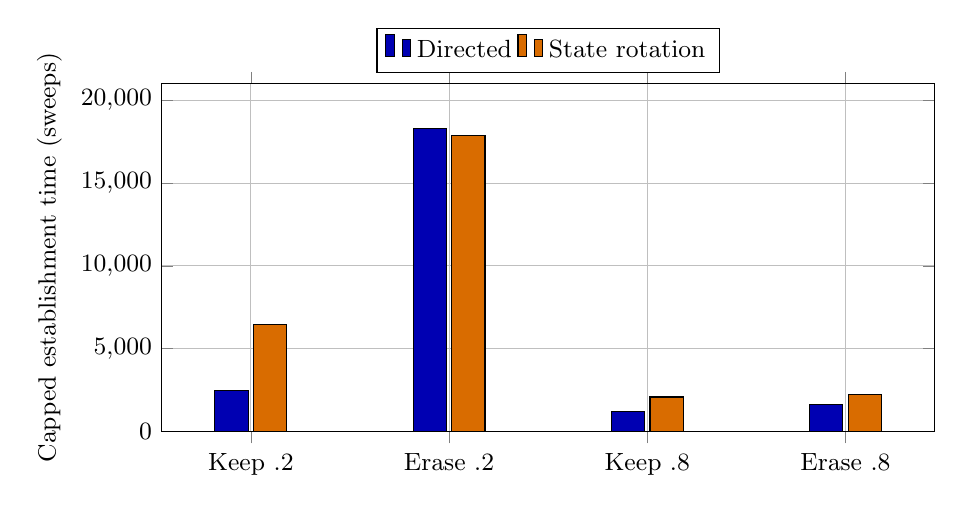
\begin{tikzpicture}\begin{axis}[width=0.94\linewidth,height=6cm,ymin=0,ymax=21000,scaled y ticks=false,ytick={0,5000,10000,15000,20000},ylabel={Capped establishment time (sweeps)},grid=major,legend style={at={(0.5,1.03)},anchor=south,legend columns=2,font=\small},tick label style={font=\small},label style={font=\small},ybar,bar width=12pt,xtick={1,2,3,4},xticklabels={Keep .2,Erase .2,Keep .8,Erase .8},enlarge x limits=0.15]\addplot[fill=blue!70!black] coordinates {(1,2480) (2,18280) (3,1210) (4,1610)};\addplot[fill=orange!85!black] coordinates {(1,6450) (2,17900) (3,2090) (4,2240)};\legend{Directed,State rotation}\end{axis}\end{tikzpicture}
\caption{Expression and learning-rate intervention after the 512th fixed-norm update. The labels specify newborn expression and $\eta_c$. Each bar includes all 20 runs; attainment counts and auxiliary zero-learning results are in Table~\ref{tab:mechanism}. The same-direction branches share their pre-intervention histories.}\label{fig:mechanism}
\end{figure}
\begin{table}[htbp]\caption{All expression-intervention conditions. D denotes directed inheritance and R denotes state-preserving randomization. Reached entries give successful runs out of 20; AUC D/R lists the two normalized occupancy areas. Times are capped at 20,000 sweeps.}\label{tab:mechanism}
\begin{center}
\small
\begin{tabular}{rlccrrc}
\toprule
$\eta_c$ & Expression & Reached D & Reached R & $\bar T_D^*$ & $\bar T_R^*$ & AUC D/R \\
\midrule
0 & Keep & 20/20 & 6/20 & 1390 & 15540 & 0.959/0.379 \\
0 & Erase & 0/20 & 0/20 & 20000 & 20000 & 0.009/0.009 \\
0.2 & Keep & 20/20 & 18/20 & 2480 & 6450 & 0.934/0.827 \\
0.2 & Erase & 6/20 & 5/20 & 18280 & 17900 & 0.702/0.649 \\
0.8 & Keep & 20/20 & 20/20 & 1210 & 2090 & 0.966/0.934 \\
0.8 & Erase & 20/20 & 20/20 & 1610 & 2240 & 0.955/0.929 \\
\bottomrule
\end{tabular}
\end{center}
\end{table}

\subsection{Continuous native writeback retains a benefit}
We next remove fixed-norm rescaling and use Equation~\ref{eq:native}. With continuous writeback, both directions establish in all 20 runs for each of the six tested $f\times\lambda$ combinations. Directed inheritance is faster in each of the 20 paired seeds within every combination, and also yields higher normalized occupancy AUC. For $f=0.5$, directed/random mean times are 2,490/4,040, 1,490/2,840, and 930/2,330 at $\lambda=0.25,0.5,1$. For $f=0.65$, they are 2,060/2,730, 1,170/1,940, and 660/1,520. All native settings and their occupancy outcomes are reported in Table~\ref{tab:native}.

The benefit therefore does not occur only under fixed-norm rescaling. This native comparison does not, however, isolate direction at equal cumulative variation: different histories produce different update magnitudes and counts. The no-writeback references become extinct in all 20 seeds for each of these two environments; this is a conditional reference outcome, not a claim that hereditary learning is always necessary for establishment.

\subsection{Stopping writeback can change the ranking}
At $f=0.65$, continuous native writeback favors directed inheritance for all three strengths, but stopping at $B=1024$ changes the outcome. At $\lambda=0.5$, directed/random attainment is 0/20 versus 17/20; at $\lambda=1$, it is 5/20 versus 20/20. At $\lambda=0.25$, neither group establishes, yet AUC is lower for directed inheritance (0.686 versus 0.734). None of these main variation groups becomes extinct. Quota-limited and continuous branches have identical update records through the 1,024th update for all 240 matched pairs, validating the common prefix of this intervention.

There is also an endpoint-specific reversal at baseline $f=0.5$, $\lambda=0.25$, and $B=1024$: directed/random attainment is 7/20 versus 20/20, and capped times are 17,790/4,900. Yet directed AUC is slightly higher (0.844 versus 0.830), while its late occupancy is lower (0.948 versus 0.988). At the auxiliary 90\% threshold both establish in all seeds; at 99\%, attainment is 0/20 versus 8/20. These observations do not support a statement that random updating is better on every metric.

\begin{figure}[htbp]\centering
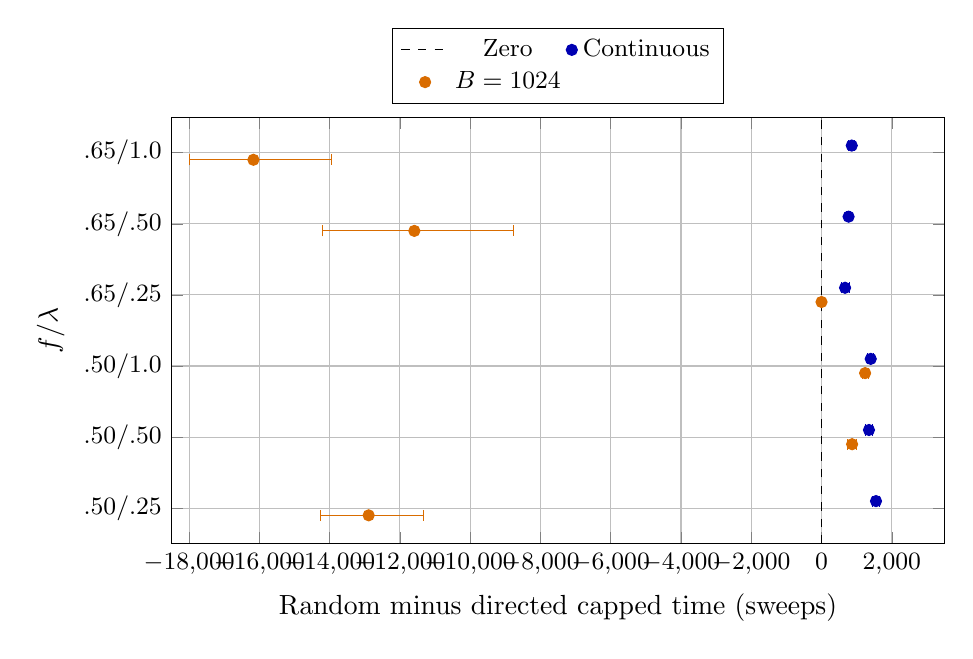
\begin{tikzpicture}\begin{axis}[width=.94\linewidth,height=7cm,xmin=-18500,xmax=3500,scaled x ticks=false,xlabel={Random minus directed capped time (sweeps)},ytick={1,2,3,4,5,6},yticklabels={$.50/.25$,$.50/.50$,$.50/1.0$,$.65/.25$,$.65/.50$,$.65/1.0$},ylabel={$f/\lambda$},ymin=.5,ymax=6.5,grid=major,legend style={at={(0.5,1.03)},anchor=south,legend columns=2,font=\small},tick label style={font=\small}]\addplot[black,dashed] coordinates {(0,.5)(0,6.5)};\addplot[only marks,mark=*,color=blue!70!black,error bars/.cd,x dir=both,x explicit] coordinates {(1550,1.1) += (100,0) -= (100,0) (1350,2.1) += (100,0) -= (100,0) (1400,3.1) += (90,0) -= (90,0) (670,4.1) += (120,0) -= (110,0) (770,5.1) += (60,0) -= (60,0) (860,6.1) += (90,0) -= (90,0)};\addplot[only marks,mark=*,color=orange!85!black,error bars/.cd,x dir=both,x explicit] coordinates {(-12890,0.9) += (1560,0) -= (1360,0) (870,1.9) += (130,0) -= (130,0) (1240,2.9) += (90,0) -= (80,0) (0,3.9) += (0,0) -= (0,0) (-11590,4.9) += (2830,0) -= (2610,0) (-16170,5.9) += (2230,0) -= (1810,0)};\legend{Zero,Continuous,$B=1024$}\end{axis}\end{tikzpicture}
\caption{Native writeback: paired differences in capped establishment time. Positive values favor directed inheritance. Points are means across 20 seed pairs; intervals are descriptive 95\% paired bootstrap intervals, without multiplicity correction. The zero difference for $f=0.65$, $\lambda=0.25$, $B=1024$ reflects complete nonattainment in both groups, not equivalence.}\label{fig:native}
\end{figure}

\begin{table}[htbp]\caption{All native variation conditions (20 seeds per direction). Each paired entry lists the directed value followed by the random value. In the Reached column, these are counts out of 20 in each group; for example, 20/20 means that both groups have 20 successful runs. $B=\infty$ denotes continuous writeback. All listed groups have zero extinctions. Late is the final-five-sample occupancy mean.}\label{tab:native}
\begin{center}
\small
\begin{tabular}{rrrcccc}
\toprule
$f$ & $B$ & $\lambda$ & Reached D/R & $\bar T^*$ D/R & AUC D/R & Late D/R \\
\midrule
0.5 & $\infty$ & 0.25 & 20/20 & 2490/4040 & 0.927/0.856 & 0.999/0.999 \\
0.5 & $\infty$ & 0.5 & 20/20 & 1490/2840 & 0.957/0.908 & 0.999/0.999 \\
0.5 & $\infty$ & 1.0 & 20/20 & 930/2330 & 0.975/0.927 & 0.999/0.999 \\
0.5 & 1024 & 0.25 & 7/20 & 17790/4900 & 0.844/0.830 & 0.948/0.988 \\
0.5 & 1024 & 0.5 & 20/20 & 2040/2910 & 0.939/0.906 & 0.990/0.998 \\
0.5 & 1024 & 1.0 & 20/20 & 1000/2240 & 0.973/0.930 & 0.998/0.999 \\
0.65 & $\infty$ & 0.25 & 20/20 & 2060/2730 & 0.970/0.917 & 0.999/0.999 \\
0.65 & $\infty$ & 0.5 & 20/20 & 1170/1940 & 0.980/0.943 & 0.999/0.999 \\
0.65 & $\infty$ & 1.0 & 20/20 & 660/1520 & 0.986/0.958 & 0.999/0.999 \\
0.65 & 1024 & 0.25 & 0/0 & 20000/20000 & 0.686/0.734 & 0.718/0.819 \\
0.65 & 1024 & 0.5 & 0/17 & 20000/8410 & 0.736/0.897 & 0.778/0.967 \\
0.65 & 1024 & 1.0 & 5/20 & 17720/1550 & 0.870/0.956 & 0.904/0.997 \\
\bottomrule
\end{tabular}
\end{center}
\end{table}

\subsection{Benefits survive common stability constraints}
The new stability seed block retains the continuous directed speed advantage in all six strength-by-energy settings under the narrower common range. Both directions establish in all runs, with no extinctions; directed inheritance is faster in every seed pair. The mean directed/random times at $f=0.5$ are 2,500/4,040, 1,610/3,040, and 1,230/3,040 for $\lambda=0.25,0.5,1$, respectively; at $f=0.65$ they are 2,030/2,810, 1,180/1,990, and 1,000/1,890. Directed AUC is also higher in each condition. The wider range and norm-only variants retain the same time ordering across their tested continuous conditions.

The unbounded random rule in this new block reaches a maximum single step of 65.381 and a maximum absolute offspring coordinate of 128.954. The norm cap limits the former but still permits coordinates up to 3.426; the narrower range limits absolute coordinates to 0.620. Thus continuous benefits do not require unbounded random drift. Nevertheless, at $f=0.65$, $\lambda=1$, bounded continuous directed/random cumulative norm sums are approximately 3,593/7,492. Same-parent geometry matching is not equal realized population-wide variation.

\subsection{The event cutoff is endogenous to reproduction}
The bounded 1,024-event comparison still reverses at $f=0.65$, $\lambda=1$: directed attainment is 0/20 and random attainment 14/20 in the stability block. Its post hoc audit finds mean quota-exhaustion times of 133.95 and 724.00 sweeps. Thus the two methods receive different temporal opportunities despite the same event quota. Stopping new writes neither deletes accumulated hereditary values nor stops lifetime learning.

The subsequent independent cutoff block repeats this dependence (Table~\ref{tab:cutoff}). The prespecified 750-sweep contrast improves the random-minus-directed capped-time difference by 15,930 sweeps [13,470,18,190] relative to the 1,024-event rule. Within the 750-sweep condition the advantage is 6,520 [4,400,8,990]. However, this change accompanies approximately 3,910 directed writes versus 1,094 random writes, so it is not a pure timing effect at equal update amounts. The early common cutoff leaves both groups unestablished, although directed AUC is higher. All four conditions have zero extinctions.

\begin{table}[htbp]\centering\small
\caption{Common-cutoff diagnostic at $f=0.65$, $\lambda=1$; 20 runs per direction. Entries list directed/random values; attainment entries are two counts, each out of 20. Failed runs retain the 20,000-sweep time cap.}\label{tab:cutoff}
\begin{tabular}{lrrrr}\toprule
Rule & Attained D/R & $\bar T^*$ D/R & AUC D/R & Mean writes D/R\\\midrule
Continuous & 20/20 & 1000/1870 & .982/.947 & 46888/47796\\
1,024 events & 0/14 & 20000/10590 & .800/.898 & 1024/1024\\
150 sweeps & 0/0 & 20000/20000 & .814/.688 & 1073/444\\
750 sweeps & 20/18 & 1000/7520 & .979/.907 & 3910/1094\\\bottomrule
\end{tabular}
\end{table}

\subsection{Matched-budget staging improves occupancy, not establishment}
All 80 fixed-step allocation runs use their full quota, giving identical cumulative norm sums of 20.48 and squared-norm sums of 0.4096. No run becomes extinct, but none reaches the primary establishment threshold. Consequently, the prespecified faster-establishment prediction is not supported, and the capped-time tie is not evidence of equivalence.

Secondary occupancy outcomes do differ (Table~\ref{tab:staging}). Staging improves directed AUC by 0.08249 [0.07842,0.08664] and random AUC by 0.00376 [$-0.02953$,0.03276]. The difference between these improvements is 0.07873 [0.05031,0.11112]. These descriptive results cannot be attributed to extra cumulative update magnitude, but they still combine timing, state coverage, geometric feasibility, and selection along diverging histories. They support a limited allocation effect rather than a successful establishment intervention.

\begin{table}[htbp]\centering\small
\caption{Fixed-step allocation ($q=0.02$, $B=1024$). Each group has 20 seeds, zero attainment and zero extinction. All groups use exactly the same event count and cumulative magnitudes.}\label{tab:staging}
\begin{tabular}{llrrr}\toprule
Schedule & Direction & AUC & Late occupancy & Mean exhaustion sweep\\\midrule
Earliest & Directed & .6786 & .7010 & 142.3\\
Earliest & Random & .6274 & .7140 & 803.7\\
Staged & Directed & .7611 & .7919 & 777.9\\
Staged & Random & .6312 & .7339 & 1416.2\\\bottomrule
\end{tabular}
\end{table}

\subsection{Ecological and numerical limits}
Fixed-norm sensitivity experiments at $B=1024$ preserve the speed ordering at lower mortality, smaller offspring energy share, and zero birth bonus (Appendix~\ref{app:robust}). At background mortality $0.01$, both directions become extinct before using the quota: average update counts are 275.8 and 225.2. At low mortality $0.0005$, even the no-writeback reference establishes in 20/20 runs. The benefit is therefore neither necessary in every environment nor sufficient under severe mortality.

In the fixed-norm high-offspring-share condition, directed/random attainment is 0/20 versus 18/20. Both survive, but directed occupancy is lower. The native continuous results show why this cannot be attributed to offspring energy share alone: the reversal depends on the update rule and cutoff as well. Higher birth and energy-death counts in the fixed-norm directed group are post hoc descriptions; their causal role has not been independently established.

Native hereditary magnitude is not matched over trajectories. For $f=0.5$, $\lambda=0.5$, and $B=1024$, the directed/random mean cumulative increment norms are about 99.10/158.09 and squared sums 13.28/30.03. Under continuous writeback at $f=0.65$, $\lambda=1$, the random squared-sum median is approximately 15,343 versus 567 for directed inheritance. The random group's mean squared increment sum, approximately 480,899, is dominated by a run whose squared sum is $9.31\times10^6$ and maximum single-step norm is approximately 1,664.48. This run is retained.

For $0\leq\lambda\leq1$, directed native inheritance is the coordinate-wise convex combination $(1-\lambda)g+\lambda\theta$. State rotation preserves candidate row geometry but not this convex-hull property. Differential stability and variation magnitude therefore limit interpretation of the original native comparison. The bounded follow-up rules out unbounded random drift as necessary for a continuous benefit, but does not decompose the original effect or equalize cumulative changes. A diagnostic replay of the large-step run passes row-scaled floating-point tolerances and reproduces its saved outputs exactly; numerical validity does not eliminate this scientific limitation.

\section{Discussion}
The strongest supported conclusion is conditional. In this artificial ecology, learned action preferences can accelerate establishment relative to a structured random alternative, and their expression in newborns can reduce the establishment delay associated with reconstructing behavior. Hereditary event allocation is also consequential: an event quota can reverse the process ordering, while common-time cutoffs change that comparison. With matched counts and magnitudes, staged release improves secondary occupancy but not the primary establishment outcome. These statements apply to different interventions and should not be collapsed into a single universal causal effect.

The control comparison provides a practical methodological lesson. Equal Euclidean magnitude alone does not preserve where a change acts. Whole-table randomization is a useful diagnostic, but can mix action direction with state allocation and reachability. Our stronger control holds more of that structure fixed, substantially changing the empirical interpretation. It is still partial matching: state-wise common values carry information, trajectories diverge, and Euclidean changes are not matched changes in action probabilities or information content. A broader control methodology would need to address these distinctions in other representations.

The expression intervention gives a more direct test than correlations between parental success and offspring success. Removing newborn contrast values while preserving the inherited table and row means changes performance; increasing the rate of lifetime adjustment compensates for much of the measured erasure loss. Nevertheless, a common state value can affect later updates, and the intervention begins at the birth that exhausts the population-wide hereditary update quota. It is a test of preference expression in that regime, not an intervention that removes all inherited learning or a complete explanation of the native-process effect.

The cutoff results also separate a genuine experimental dependence from a biological explanation. The quota is externally imposed on hereditary events; there is no modeled metabolic charge for writing a parameter. Thus the evidence does not establish that natural energetic limits generate the same cutoff, nor that rapid early establishment reduces long-term evolvability. High occupancy is itself only one population-level endpoint. We observe reversals without population extinction, and in one native condition AUC and establishment time rank methods differently.

Several limitations constrain transfer beyond this study. The ecology and learner are deliberately simple; the coarse-binning analysis shares the same simulator. The reward is engineered and division feasibility is an explicit input. Mortality is stochastic rather than an age-based developmental process. Independent mutation is absent from the core comparisons. All final formal conditions have 20 seeds, and descriptive intervals are not corrected for the number of comparisons. The sequence follows exploratory model development, including an earlier learner whose reward structure was revised, rather than a single prospectively registered program. Neither the initial exploratory phase claims nor persistent-novelty proxies are treated as confirmation of evolvability here.

The symmetric stability and allocation diagnostics narrow these alternatives without establishing a universal explanation. In particular, the matched-budget experiment did not confirm its primary prediction; a secondary occupancy effect should not be relabeled as faster establishment. Testing a prespecified mechanism in an independently implemented learner remains outside the core evidence presented here.

\section{Conclusion}
Inherited learning should be evaluated against controls that distinguish update direction from structure and magnitude. In the tested artificial ecology, this distinction reduces a large apparent attainment advantage to a more conditional speed benefit. Newborn preference erasure and learning-rate compensation support a role for repeated learning, while symmetric stability constraints retain continuous benefits and allocation diagnostics expose different benefit boundaries. Matched-budget staging affects occupancy but does not achieve establishment in the tested small-step regime. These results support a bounded mechanism study of inherited action preferences, not a general law of evolution or an unqualified advantage of acquired-trait inheritance.

\section*{Data and code availability}
Code, protocols, formal seed-level results, population traces, summaries, and validation records are available at \url{https://github.com/deep-geo/inherited-learning-ecology}. Full per-event logs are retained separately and are available from the corresponding author on request. No permanent archive DOI has yet been assigned.

\section*{Author declarations}
Xuening Wu conceived and directed the study and prepared the manuscript. This research received no funding. The author declares no competing interests. The experiments are computational simulations, with no human participants, animals, or biological cell experiments. Responsibility for the scientific content rests with the author.

\appendix
\section{Additional ecological outcomes}\label{app:robust}
Table~\ref{tab:robust} reports the six fixed-norm sensitivity settings, each at $B=1024$. The baseline mortality is $0.002$, offspring share $0.5$, and birth bonus $0.2$. Each alternative changes one of these settings: mortality to $0.0005$ or $0.01$, offspring share to $0.35$ or $0.65$, or bonus to zero. Changing offspring share also changes the complementary parent share. No-writeback results and individual runs are retained in the accompanying data, not pooled across settings. All high-mortality failures are retained despite unused quota.
\begin{table}[htbp]\caption{Ecological sensitivity. Paired entries list directed and random values; each group has 20 seeds. Reached and Extinct entries are two counts, each out of 20, not fractions. The high-mortality capped-time tie reflects nonattainment in both groups, not equivalence.}\label{tab:robust}
\begin{center}
\small
\begin{tabular}{lcccc}
\toprule
Setting & Reached D/R & $\bar T^*$ D/R & Extinct D/R & AUC D/R \\
\midrule
baseline & 20/20 & 1460/3190 & 0/0 & 0.960/0.895 \\
low death & 20/20 & 1000/1730 & 0/0 & 0.978/0.959 \\
high death & 0/0 & 20000/20000 & 20/20 & 0.002/0.002 \\
low child energy & 20/20 & 1530/3160 & 0/0 & 0.953/0.903 \\
high child energy & 0/18 & 20000/5290 & 0/0 & 0.814/0.908 \\
no birth bonus & 20/20 & 2160/3560 & 0/0 & 0.931/0.881 \\
\bottomrule
\end{tabular}
\end{center}
\end{table}

\section{Reproducibility and provenance}
Codex, a generative AI tool, assisted with simulation code and execution, analysis, literature discovery, figures, and manuscript preparation. The author is responsible for the scientific content. The numerical and implementation checks described below document the validation performed; AI assistance is not independent verification.

Simulation code is written in C++17 with separate pseudorandom streams for ecological events, independent noise, direction generation, and measurements. Seeds and source snapshots are included per stage. Matched seeds align initial conditions and random-stream initialization, but do not enforce identical encounters after trajectories diverge. Source and protocol hashes were recorded by the experiment runners. Existing checks include population accounting, resource bounds, energy split conservation, geometry preservation, zero-learning and zero-writeback comparisons, and exact replay of representative outputs.

The zero-learning check compares writeback variants within the same learning-rate setting, not zero learning against learning without writeback. An initially incorrect implementation-check comparison was corrected before the native formal batch; the failed diagnostic is retained in its validation records. The large native random-update replay required a scale-relative numerical tolerance rather than the original absolute $10^{-10}$ row-norm threshold. Its maximum reported absolute discrepancy was $4.66\times10^{-10}$; a diagnostic run with row-scaled tolerances reproduced all seven archived output types byte for byte.

For the initial manuscript synthesis, all 1,840 formal population traces were independently re-read to recompute attainment at 90\%, 95\%, and 99\%, capped times, normalized occupancy AUC, late occupancy, and extinction. These values agree with the archived seed summaries. This is a data-to-manuscript consistency check, not an independent reimplementation or a new simulation experiment. The original paired bootstrap intervals are retained. Development and replay rows are excluded from formal effect estimates. The 1,440 subsequent formal runs underwent corresponding population, energy, update-ledger, geometry, and bound checks. The cutoff implementation was checked against the preceding simulator with its new options disabled, and fixed-step release checks verified all realized quotas and magnitudes. The new seed blocks were not extended after outcome inspection.

\section{Scope of the literature comparison}
The related-work assessment uses targeted searches and primary texts available through 30 September 2026. It is not a systematic review and does not substantiate a first-ever claim. The 2023 robot preprint and its journal publication are treated as one work. The Bayesian-optimization sample-inheritance work is cited by its verified 2026 arXiv version, although an author data record exists from 2025; the upload date is not asserted to be its earliest dissemination. The two other 2026 robot works are cited as preprints without asserting final conference acceptance. Closely related effects and mechanisms are acknowledged rather than recast as newly discovered principles.

\begin{thebibliography}{10}
\bibitem{hinton1987} G. E. Hinton and S. J. Nowlan. How learning can guide evolution. \emph{Complex Systems}, 1:495--502, 1987. \url{https://www.cs.toronto.edu/~hinton/absps/evolution.htm}.
\bibitem{rivoire2014} O. Rivoire and S. Leibler. A model for the generation and transmission of variations in evolution. \emph{Proceedings of the National Academy of Sciences}, 111:E1940--E1949, 2014. \href{https://doi.org/10.1073/pnas.1323901111}{doi:10.1073/pnas.1323901111}.
\bibitem{jelisavcic2019} M. Jelisavcic, K. Glette, E. Haasdijk, and A. E. Eiben. Lamarckian evolution of simulated modular robots. \emph{Frontiers in Robotics and AI}, 6:9, 2019. \href{https://doi.org/10.3389/frobt.2019.00009}{doi:10.3389/frobt.2019.00009}.
\bibitem{luo2023} J. Luo, K. Miras, J. Tomczak, and A. E. Eiben. Enhancing robot evolution through Lamarckian principles. \emph{Scientific Reports}, 13:21109, 2023. \href{https://doi.org/10.1038/s41598-023-48338-4}{doi:10.1038/s41598-023-48338-4}.
\bibitem{aguilar2019} L. Aguilar, S. Bennati, and D. Helbing. How learning can change the course of evolution. \emph{PLOS ONE}, 14:e0219502, 2019. \href{https://doi.org/10.1371/journal.pone.0219502}{doi:10.1371/journal.pone.0219502}.
\bibitem{thomsen2023} K. R. Thomsen and S. Rasmussen. Dynamics of Darwinian versus Baldwinian versus Lamarckian evolution. \emph{arXiv:2305.00491}, 2023. \url{https://arxiv.org/abs/2305.00491}.
\bibitem{debruinSamples} K. E. de Bruin, K. Glette, and K. O. Ellefsen. Integrating sample inheritance into Bayesian optimization for evolutionary robotics. \emph{arXiv:2601.03813}, 2026. \url{https://arxiv.org/abs/2601.03813}.
\bibitem{debruinDynamic} K. E. de Bruin, K. Glette, and K. O. Ellefsen. Lamarckian inheritance in dynamic environments: How key variables affect evolutionary dynamics. \emph{arXiv:2605.15769}, 2026. \url{https://arxiv.org/abs/2605.15769}.
\bibitem{muff2026} J. R. Muff, K. Miras, and A. E. Eiben. Limits of Lamarckian evolution under pressure of morphological novelty. \emph{arXiv:2604.15854}, 2026. \url{https://arxiv.org/abs/2604.15854}.
\bibitem{benito2026} I. Benito, J. F. Lutzeyer, and B. Doerr. A fresh look at Lamarckian evolution and the Baldwin effect. \emph{arXiv:2605.28703}, 2026. \url{https://arxiv.org/abs/2605.28703}.
\end{thebibliography}
\end{document}
